\begin{fullwidth}
\chapter[Scenario planning tools and reports for the covid-19 pandemic]{Scenario planning tools and reports for \\the covid-19 pandemic}
\label{sec:covid-pipeline-reports}
  \end{fullwidth}
The ongoing Coronavirus disease 2019 (COVID-19, previously nCov) pandemic originated in Wuhan, China at the end of year 2019. The pathogen here is a virus, the severe acute respiratory syndrome coronavirus SARS-CoV-2, which upon infections might cause a wide variety of symptoms all accross range of severity. With 4.07\textsc{M} confirmed deaths and 190\textsc{M} confirmed cases as of July 2021, we are living through one of the deadliest pandemic in history.

 All around the world, the response has mobilized scientists, public-health and medical professionals and decision-makers. Over the last year and a half, a considerable body of evidence has accumulated\sidenote[][-3\baselineskip]{With more than 190'000 peer-reviewed papers and many more preprints, website and reports published at the time of writing. Estimation from: \fullcite{COVID-19OpenAccessProject:LivingEvidenceCOVID19:2020}}. For this reason, we do not endeavour a literature review of the current (and evolving) understanding of COVID-19, nor the modeling studies which have informed the response. 

 This chapter presents some modeling works tailored for the response to COVID-19. While the COVID Scenario Pipeline is an ongoing project, we present it as it was in the early stage, taking a perspective from around July 2020. The state of knowledge on the SARS-CoV-2 and COVID-19 was very rapidly expanding, and the present chapter highlights the challenges of dealing with such uncertainties. 

%We focus on details dealing with the uncertainties that caraterize disease emergences.
\vspace{\baselineskip}
\section{The COVID Scenario Pipeline}

The COVID Scenario pipeline\sidenote{\url{github.com/HopkinsIDD/COVIDScenarioPipeline}} is being developed by the Johns Hopkins University Infectious Disease Dynamics COVID-19 Working Group. 

The pipeline is a flexible modeling framework that projects epidemic trajectories and healthcare impacts under different suites of interventions in order to aid in scenario planning. The model is generic enough to be applied to different spatial scales given shapefiles, population data, and COVID-19 confirmed case data. The pipeline is constituted of multiple components, which may be characterized as follows: 1) epidemic seeding; 2) disease transmission and non-pharmaceutical intervention scenarios; 3) calculation of health outcomes (hospital and ICU admissions and bed use, ventilator use, and deaths); and 4) summarization of model outputs.
 Other parts of the pipeline not described in this thesis\footnote[][-4\baselineskip]{Including airport importation, which was especially important in early 2020, report generation, config writing, inference, analysis, submission, see \eg \url{github.com/HopkinsIDD/COVIDScenarioPipeline} and \url{github.com/HopkinsIDD/covidImportation}}, but a previous version of the ever evolving pipeline has been described in:
\longfullcite{Lemaitre:ScenarioModelingPipeline:2021}\footnote[][-2\baselineskip]{Where Kyra H. Grantz, Joshua Kaminsky, Hannah R. Meredith, Shaun A. Truelove and I contributed equally.}.
\begin{figure*}[!htb]%[width = .7\textwidth]
    \centering
    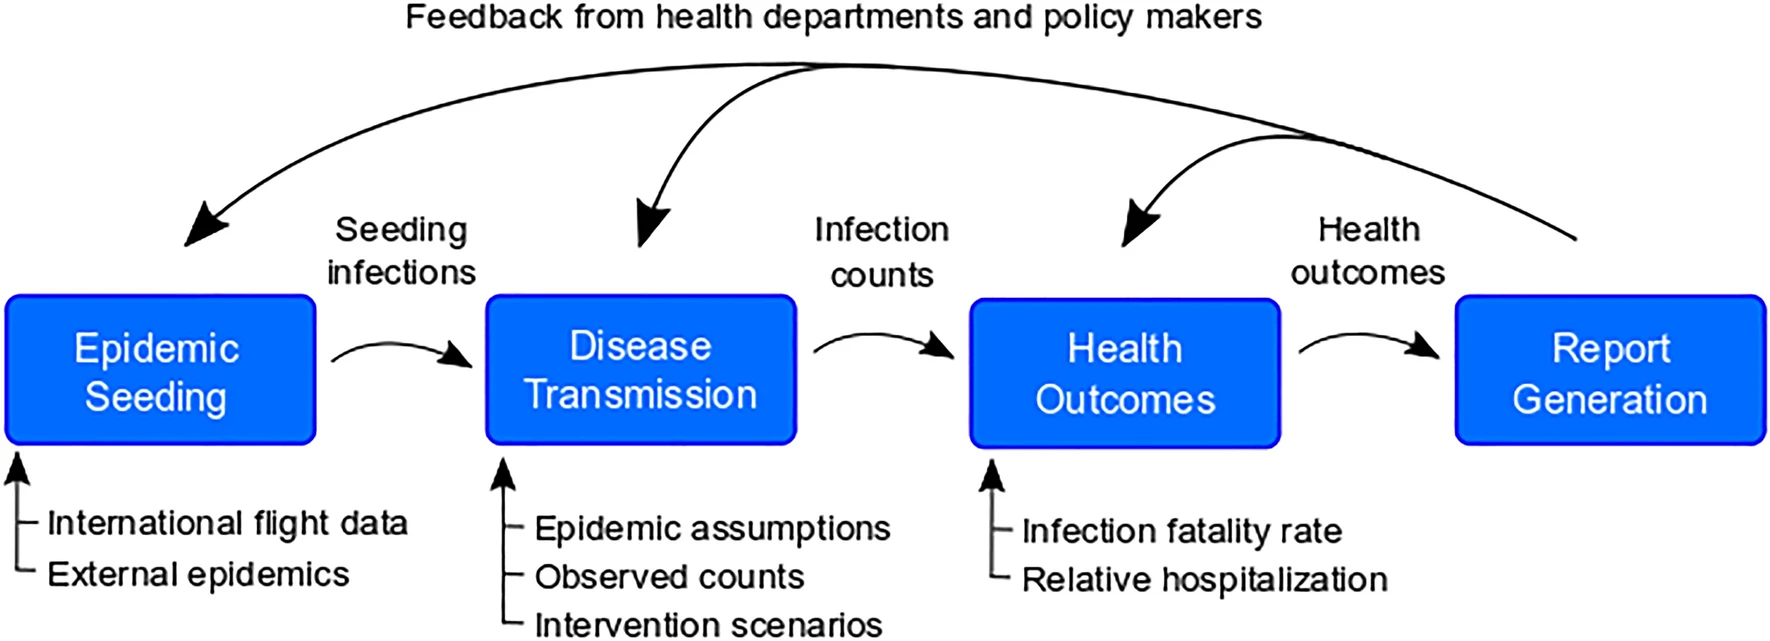
\includegraphics{fig_pipeline/fig1a}
    \caption[The four modules of the pipeline]{Overview of the four modules of the pipeline.}
    \label{fig:pipeline-modules}
\end{figure*}

\subsection{Disease transmission model}
The model for SARS-CoV-2 transmission is entirely configurable to any compartment model following an arbitrary transition graph, allowing for multi-strain, age-stratified or vaccination models. It takes as input a demographic and spatial setup\footnote{\ie a mobility matrix and spatial nodes populations}, the timeseries of imported contagious or incubating individuals from the epidemic seeding module. Then, it simulates the transmission of SARS-CoV-2 under the different exogenous modifiers of transmissions (NPIs, variants, seasonality effects). 

Sole two parameters are necessary to caraterize the dynamics and final size of an epidemic. A common choices of these two, because they are observable, are the serial interval $SI$ and the basic reproductive number $R_0$\footnote{\fullcite{Wallinga:HowGenerationIntervals:2007}}.

The serial interval represents which is the interval between two subsequent infections. For SARS-CoV-2, the serial interval was estimated to be in range $6.5-8.2$\cite[][Table S4]{Bi:EpidemiologyTransmissionCOVID19:2020}. 

The basic reproductive number $R_0$ -- the number of newly infected caused by an infecteds in a fully susceptible population, has been estimated in the range 2 -- 3 \footnote{From \fullcite{Riou:PatternEarlyHumantohuman:2020}. This very early work also characterize $R_0$ and the dispersion of the number of secondary cases as important epidemic characteristic}.



We draw uniformly from this range, and we solve
$SI = \frac{1}{2}(\frac{1}{\gamma})+\frac{1}{\sigma}$ for the inverse of the total infectious period, $\gamma$.

The basic reproductive number $R_0$ -- the number of newly infected caused by an infecteds in a fully susceptible population, is drawn for each simulation and we obtain parameter beta from
$\beta= R_0 \cdot \gamma$.

We present below the initial model built for scenario planning, and used until June 2020. This initial model is simple spatial $S\longrightarrow E \longrightarrow I \longrightarrow R$ model. In practice, we used $k = 3$ compartments of infected, $I_1, I_2, I_3$ in order to have an infectious period shaped as Erlang distribution.



Then the rates of the different compartments are given in the table below:
\begin{table}
    \centering
    \begin{tabular}{ccc}
\toprule
Transition & rate parameter &Unit \\
 \midrule
$S\longrightarrow E$  &   $\beta = R_0 \cdot \gamma$  & d$^{-1}$\\
$E\longrightarrow I_1$ & $\sigma = \frac{1}{5.2}$         & d$^{-1}$\\
$I_1\longrightarrow I_2$ & $\gamma_1 = \gamma \cdot k$ & d$^{-1}$\\
$I_2\longrightarrow I_3$ & $\gamma_1 = \gamma \cdot k$ & d$^{-1}$\\
$I_3\longrightarrow R$ & $\gamma_1 = \gamma \cdot k$&d$^{-1}$\\
\bottomrule
\end{tabular}
\caption{Transitions rate parameters for the pipeline}
     \label{tab:survpars}
\end{table}


The model is fixed time step, and the transitions (without mobility here) at each time step
$\Delta t$ are: 

\begin{eqnarray}
p_{expose} &=&  1 - \exp(-\Delta t \cdot FOI) \\
p_{infect} &=& 1 - \exp(-\Delta t \cdot \sigma)\\
p_{recover} &=& 1 - \exp(-\Delta t \cdot \gamma)
\end{eqnarray}

At each time step, we draw in a binomial distribution, e.g 
\begin{equation}
N_{I_1\longrightarrow I_2}(t) = \text{Binom}(I_1, 1 - \exp(-\Delta t \cdot \gamma_1))
\end{equation}

The force of infection without mobility is defined as: 

\begin{equation}
FOI = \beta \frac{(I_1 + I_2 + I_3)^\alpha}{H} 
\end{equation}

where $\alpha$ is a coefficient that dampens disease transmission when its value is below 1, thus more accurately representing non-homogeneous mixing in the population. Although we were unable to find $\alpha$ estimates for SARS-CoV-2, we expect disease transmission to be similar to that of other respiratory diseases and typical estimated values for $\alpha$ for respiratory diseases range from 0.87 to 0.97.

In our model, individuals move from one node to another. A mobility matrix $M$ where
$M(o,d)$ is the amount of individuals moving daily from origin $o$ to
destination $d$. At each time step, and for each $(o,d)$ pair, we draw a force of infection 
for node $i$ to account for mobility:
\begin{fullwidth}
	
\begin{equation}
FOI_i = \left(1 - \sum_{j\neq i} p_{away} \frac{M_{i,j}}{H_i} \right) \cdot \beta_i(t) \frac{(I_1^{i} + I_2^{i} + I_3^{i})^\alpha}{H_i} +  \sum_{j \neq i} \left(p_{away} \frac{M_{i,j}}{H_i} \cdot \beta_j(t) \frac{(I_1^j + I_2^j + I_3^j)^\alpha}{H_j} \right)
\end{equation}
\end{fullwidth}

with $p_{away}$ the percent of the time individuals that move spend away; $p_{away} \approx 0.5$ in the case of commuting. $H_i$ is the population of node $i$. Then, the transition is:

\begin{equation}
N_{S_i \longrightarrow I_1^{i}}(t) = \text{Binom}(S^i, 1 - \exp(-\Delta t \cdot FOI_i))
\end{equation}

\paragraph{Non-Pharmaceutical interventions} and other transmission alter parameter $\beta$. The copounded effects on transmission of the reductions of the $k$ intervention in place at time $t$ and node $i$ is:
\begin{equation}
	\beta_i'(t) =  \beta_i(t) \cdot  \prod_k \left(1-r_k(t) \right) \label{eq:npi}% _{i=1}^{N_{\text{mod(t)}}
\end{equation}
Several interventions templates are provided, and the copounding  of interventions is with either multiplicative (as in Equation \eqref{eq:npi}) or additive copounding depending on the parameters. 

\paragraph{Health Outcomes} are computed on top of the incidence for each compartments. Each outcomes $O$  is specified from a source incidence $S$, with a delay $\Delta$ and a duration $D$:

 \begin{algorithm}[H]
\SetAlgoLined
  \SetKwInOut{Input}{inputs}
  \SetKwInOut{Output}{output}
  \SetKwProg{FindAnMFS}{FindAnMFS}{}{}
  \FindAnMFS{$(Q,D)$}{
\KwResult{Write here the result }
\Input{A failing query $Q = t_1 \wedge \dots \wedge t_n$; an \texttt{RDF} database $D$}
 \Output{An \texttt{MFS} denoted by $Q^*$}
draw $\Delta$ from config distribution\;
draw $D$ from config distribution\;
\ForEach{$t$ in $t_i, t_i+1, ..., t_f$}{
$O[t+\Delta:t+\Delta+D]\leftarrow O[t+\Delta:t+\Delta+D] + \text{Binom}(S[t], p_{O\mid S})$\;}
 }
 \caption{Computations of health outcomes}
\end{algorithm}
and the rates are ajusted the different population-based risk, as further described in\cite{Lemaitre:ScenarioModelingPipeline:2021}.



The epidemic tranmssion model, the intervention module and the outcome calculation are implemented in python, just-in-time compiled to machine code using Numba\cite{Lam:NumbaLLVMbasedPython:2015}. The team working on the pipeline has brought many improvements, both computational and conceptual, that have enabled the pipeline to remain useful in 2021. 

\section{Example of scenario planning report for Canton de Vaud}
The COVIDScenarioPipeline has been used in different settings (list). We present here a report produced on April 9, 2020, for Canton de Vaud main hopital, CHUV. The inference module of the pipeline did not exist yet, so scenario projects were generated using a simple particle filter like methods\footnote{This is a collaboration between many different actors further analysis and algorithm developed with Dr. Perez-Saez.}
3. Interaction with public-health decision maker. Usefulness of modeling

% pagecommand adds page numbers,  need package pdfpages

 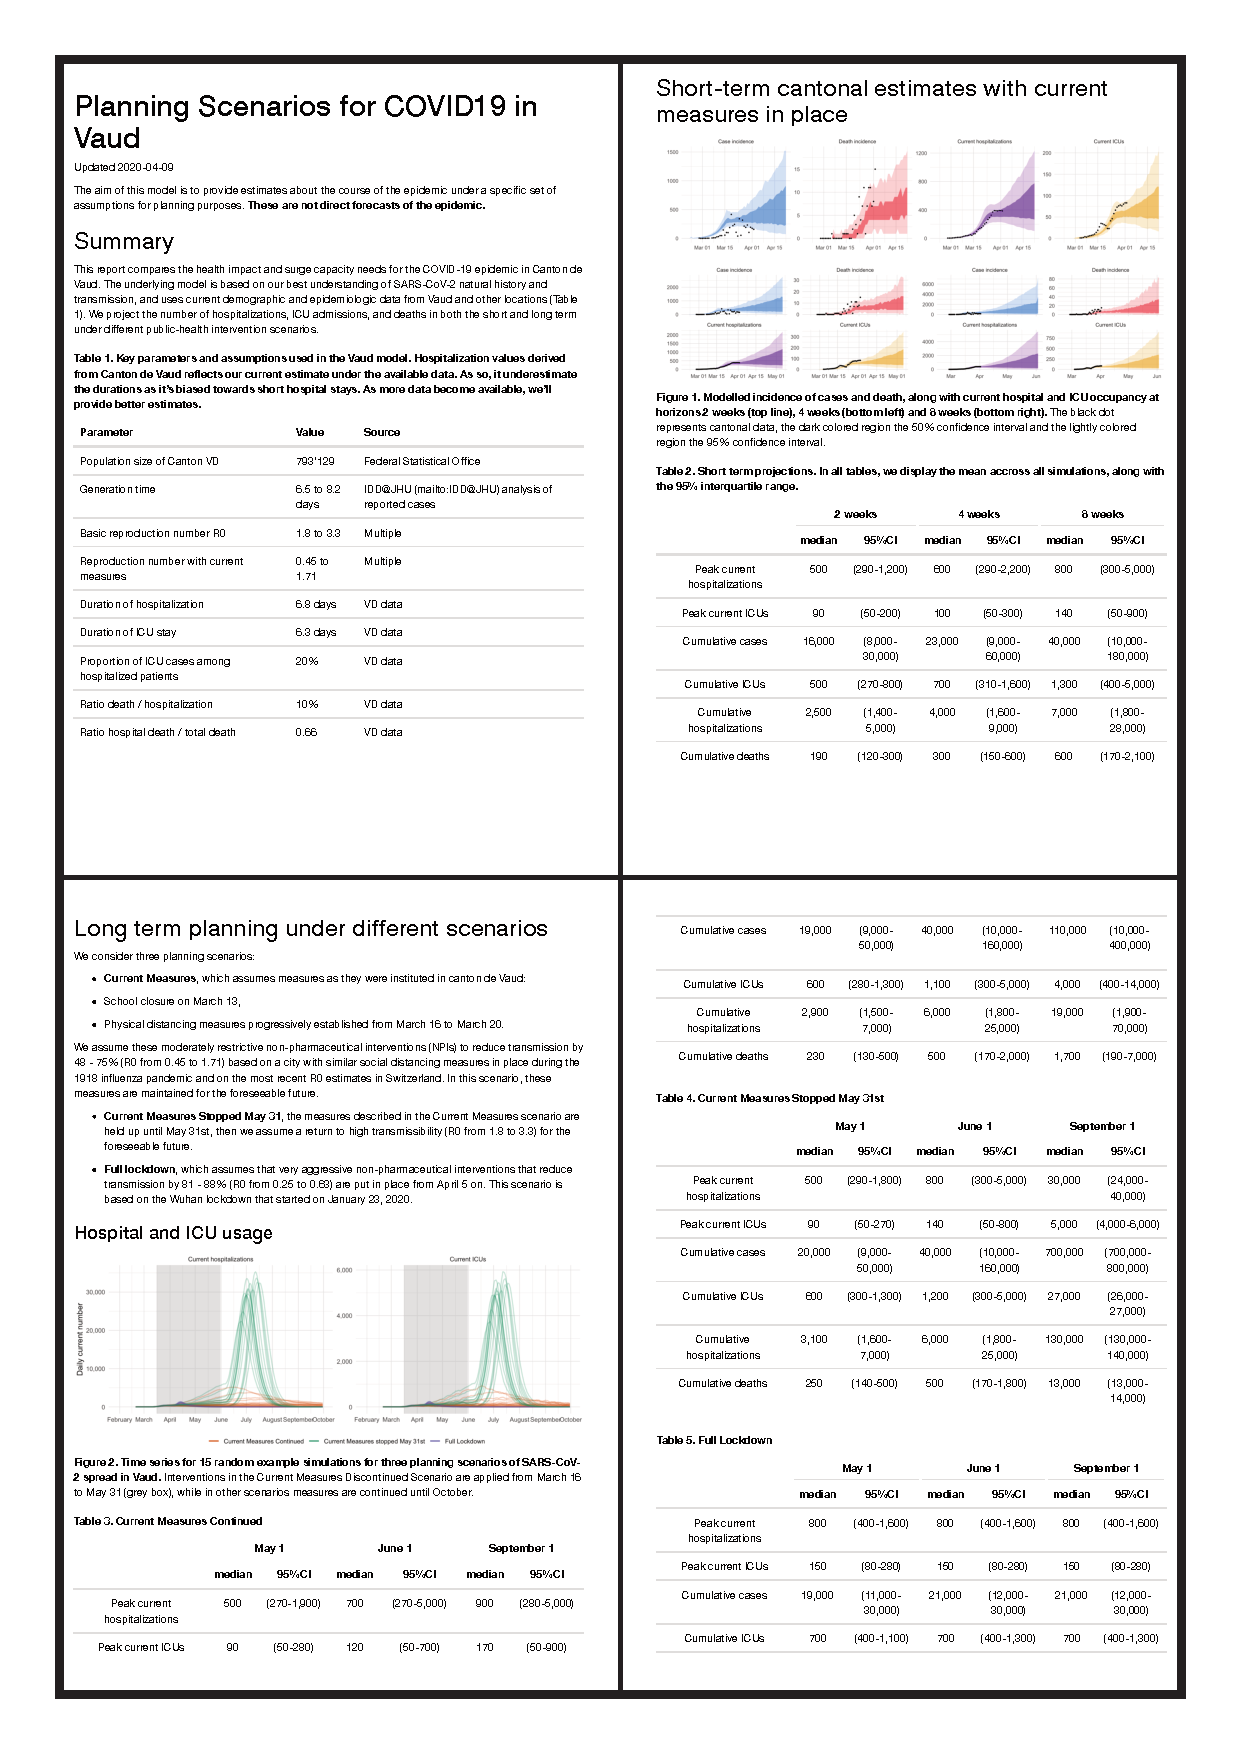
\includepdf[pages=-, pagecommand={\thispagestyle{empty}}]{fig_pipeline/planning_mod.pdf}

\section{Model Parameters from truncated data}
While collaborating with CHUV on these reports, we had access to precise hospitalization data. It allowed us to refine our estimates\cite{Rees:COVID19LengthHospital:2020}. While we used naively the truncated data. This section is published in the supplementary material of
\fullcite{Lemaitre:AssessingImpactNonpharmaceutical:2020}.
\begin{figure}[!htb]% [width = .7\textwidth]
    \centering
        \caption[Age distribution of patients hospitalized for COVID-19 in the canton of Vaud]{Age distribution of patients hospitalized for COVID-19 in the canton of Vaud up to April 14. Hospitalized individuals are divided in two subgroups depending on if they were treated in ICU (left) or not (right) during their stay. Moreover, only the 777 patients with known outcome are displayed here. We highlight the outcome:  either death (orange) or discharge/transfer to another hospital (blue).}
    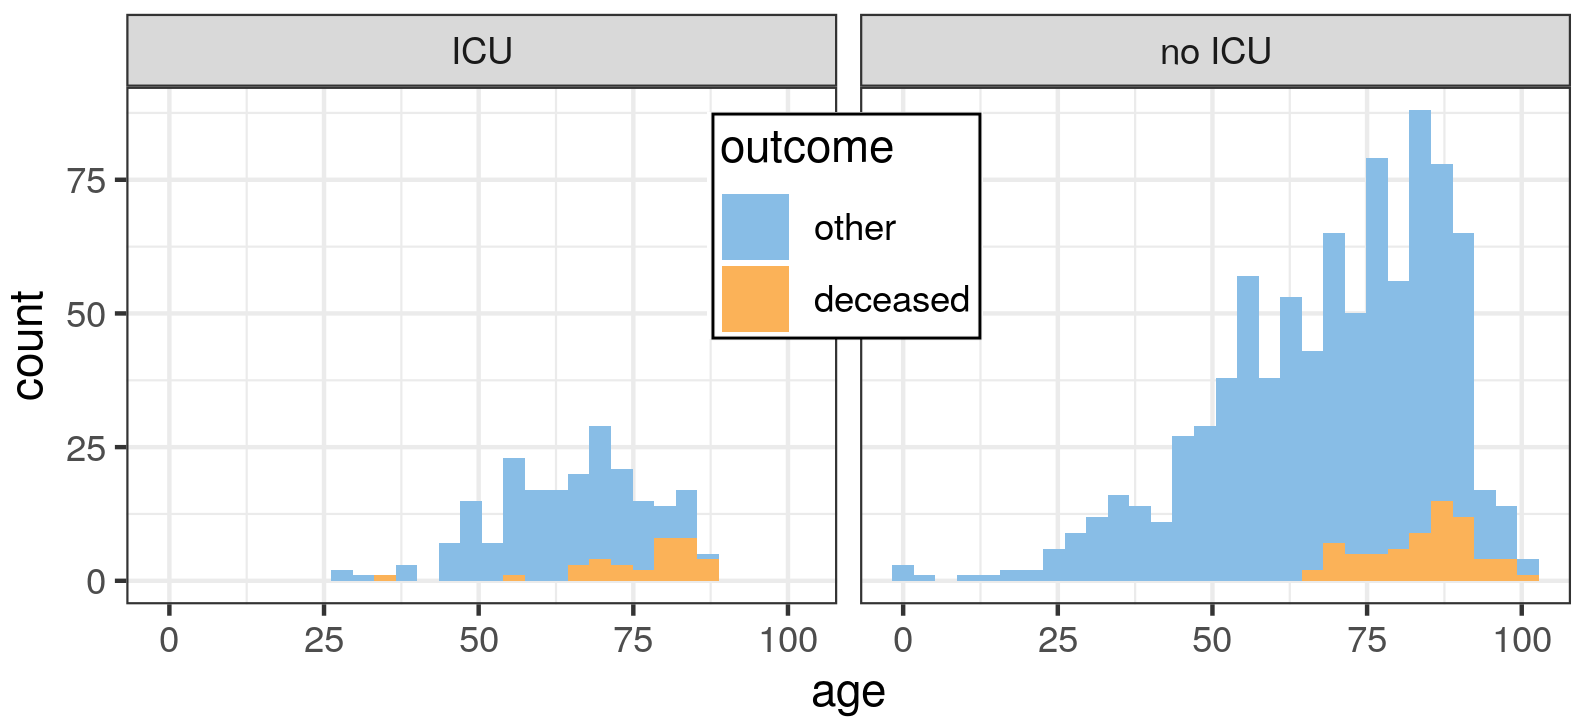
\includegraphics{fig_covid-switzerland-npi/fig_supp/VD_hist_age_mod.png}
    \label{fig:vdage}
\end{figure}
\begin{figure}[!htb]
    \centering
    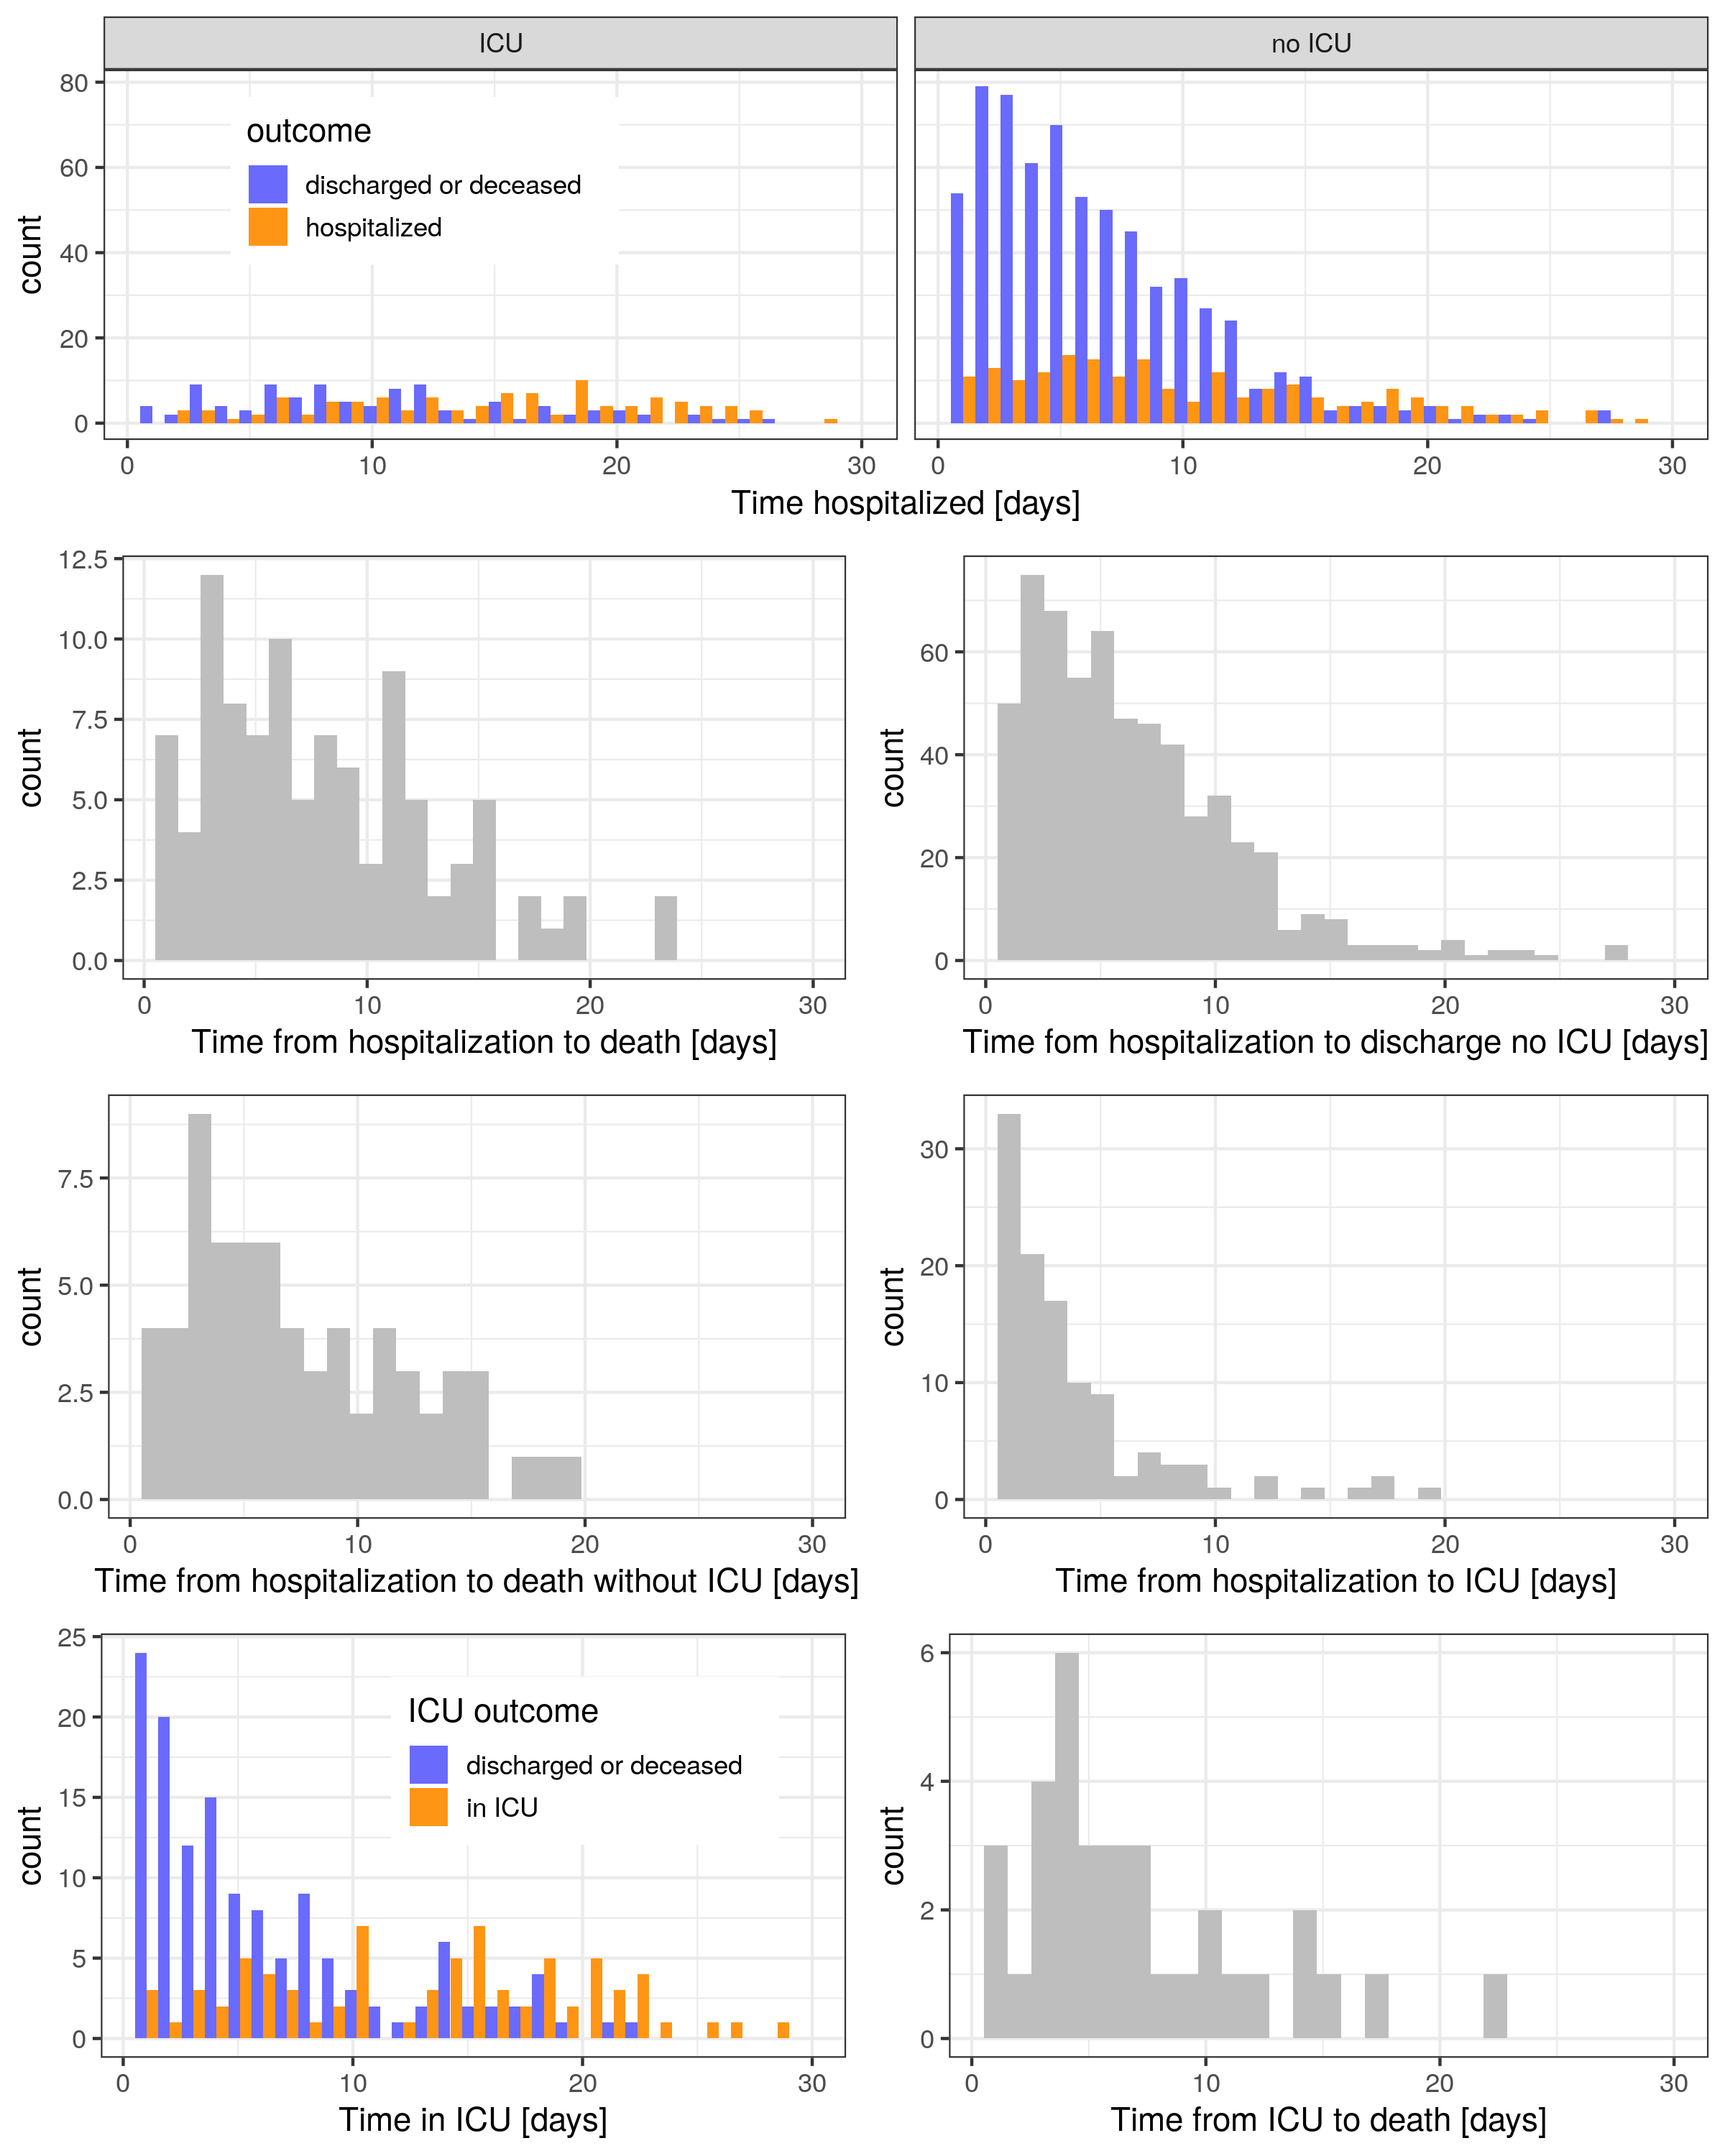
\includegraphics{fig_covid-switzerland-npi/fig_supp/VD_times.png}
    \caption[Key data of hospitalization events in canton de Vaud]{Data from canton de Vaud showing times to key hospitalization events. In order to perform this analysis, we split patients in two categories: those who did not go through ICU during their stay and those who did. From left to right, top to bottom: total length of hospital stay for patients that went to ICU, then similarly for patient that did not. Then we show the time to death for all patients, followed by both the time to discharge and to death for non-ICU patients. The last three graphs concerns ICU patients and detail ICU focused estimate: time from hospitalization to ICU, time in ICU and time from ICU to death. When meaningful, we show both currently hospitalized patient (orange) and already out-of-hospital patients (blue).}
    \label{fig:vdtimes}
\end{figure}


We had access to individual-level data from 1093 patients hospitalized in the canton of Vaud up to April 14, 2020. Of all patients, 41\% (448/1093) were female and 59\% were male (645/1093) with a median age of 70 years (Supplementary Material, SM, Figure~\ref{fig:vdage}). Of all the hospitalized cases, 20\% (214/1093) required use of an Intensive Care Unit (ICU).


Of 777 patients with a known outcome on April 14, 104 died (13\%). 
We estimate the hospitalized Case Fatality Ratio (hCFR) by adjusting for the distribution of time hospitalization to death accounting for the fact that outcomes have not been yet observed for all patients (right-censoring). To account for multiple outcomes (death and discharge), we implement a parametric competing risk survival model similar to that of\cite{Ghani:MethodsEstimatingCase:2005}. We follow a Bayesian approach proposed in\cite{Bellot:TreebasedBayesianMixture:2018} that enables us to fit parametric distributions to times to events using accelerated failure models. This method allows for the joint estimation of the probability of each event type and the distributions of times to events. In this case we are interested in the probability of death, i.e. the hCFR. A COVID-19 modeling study in France identified mixtures of probabilities of times to death, with a group dying faster with exponentially-distributed times and one dying slower\cite{Salje:EstimatingBurdenSARSCoV2:2020}. We therefore extend the Bayesian survival framework to test for mixture in times to death and recovery. We did not take into model patients being discharged from ICU and subsequently dying which was the case for 4/138 patients with known outcome. We neither accounted for multiple ICU stays per patient since we did not have that information. We fit both Gamma and Log-Normal distributions separately to patients that did not go into ICU, and patients that did. For the former, we model times from hospitalization to death or discharge, and for the latter times from ICU entry to both outcomes. Models were fit with Stan\cite{Carpenter:StanProbabilisticProgramming:2017}, and selection was done using Bayesian leave-one-out cross-validation\cite{Vehtari:PracticalBayesianModel:2017}. \\
\begin{figure}[!htb]
    \centering
        \caption[Survival functions of death and discharge for hospitalized patients and patients in ICU][-3\baselineskip]{Survival functions of death and discharge for hospitalized patients and patients in ICU. The lines represent the mean estimated cumulative probability of dying (full) and 1 minus the cumulative probability of discharge (dotted) estimated with non-parametric (Aalen-Johansen estimator, shading gives the 95\% CI) and parametric (assuming gamma and log-normal distributions, shading indicate the 95\% CrI) methods. Time is in days from hospitalization for patients that did not require ICU, and time from ICU admission for those that did. The point at which the lines join represents the probability that the final outcome is death, which was estimated to be 28.1\% (95\% CrI: 16.4-40.9) for patients in ICU and 13.0\% (95\% CrI: 9.9-16.6) for patients not requiring ICU based on the log-normal distribution.}
    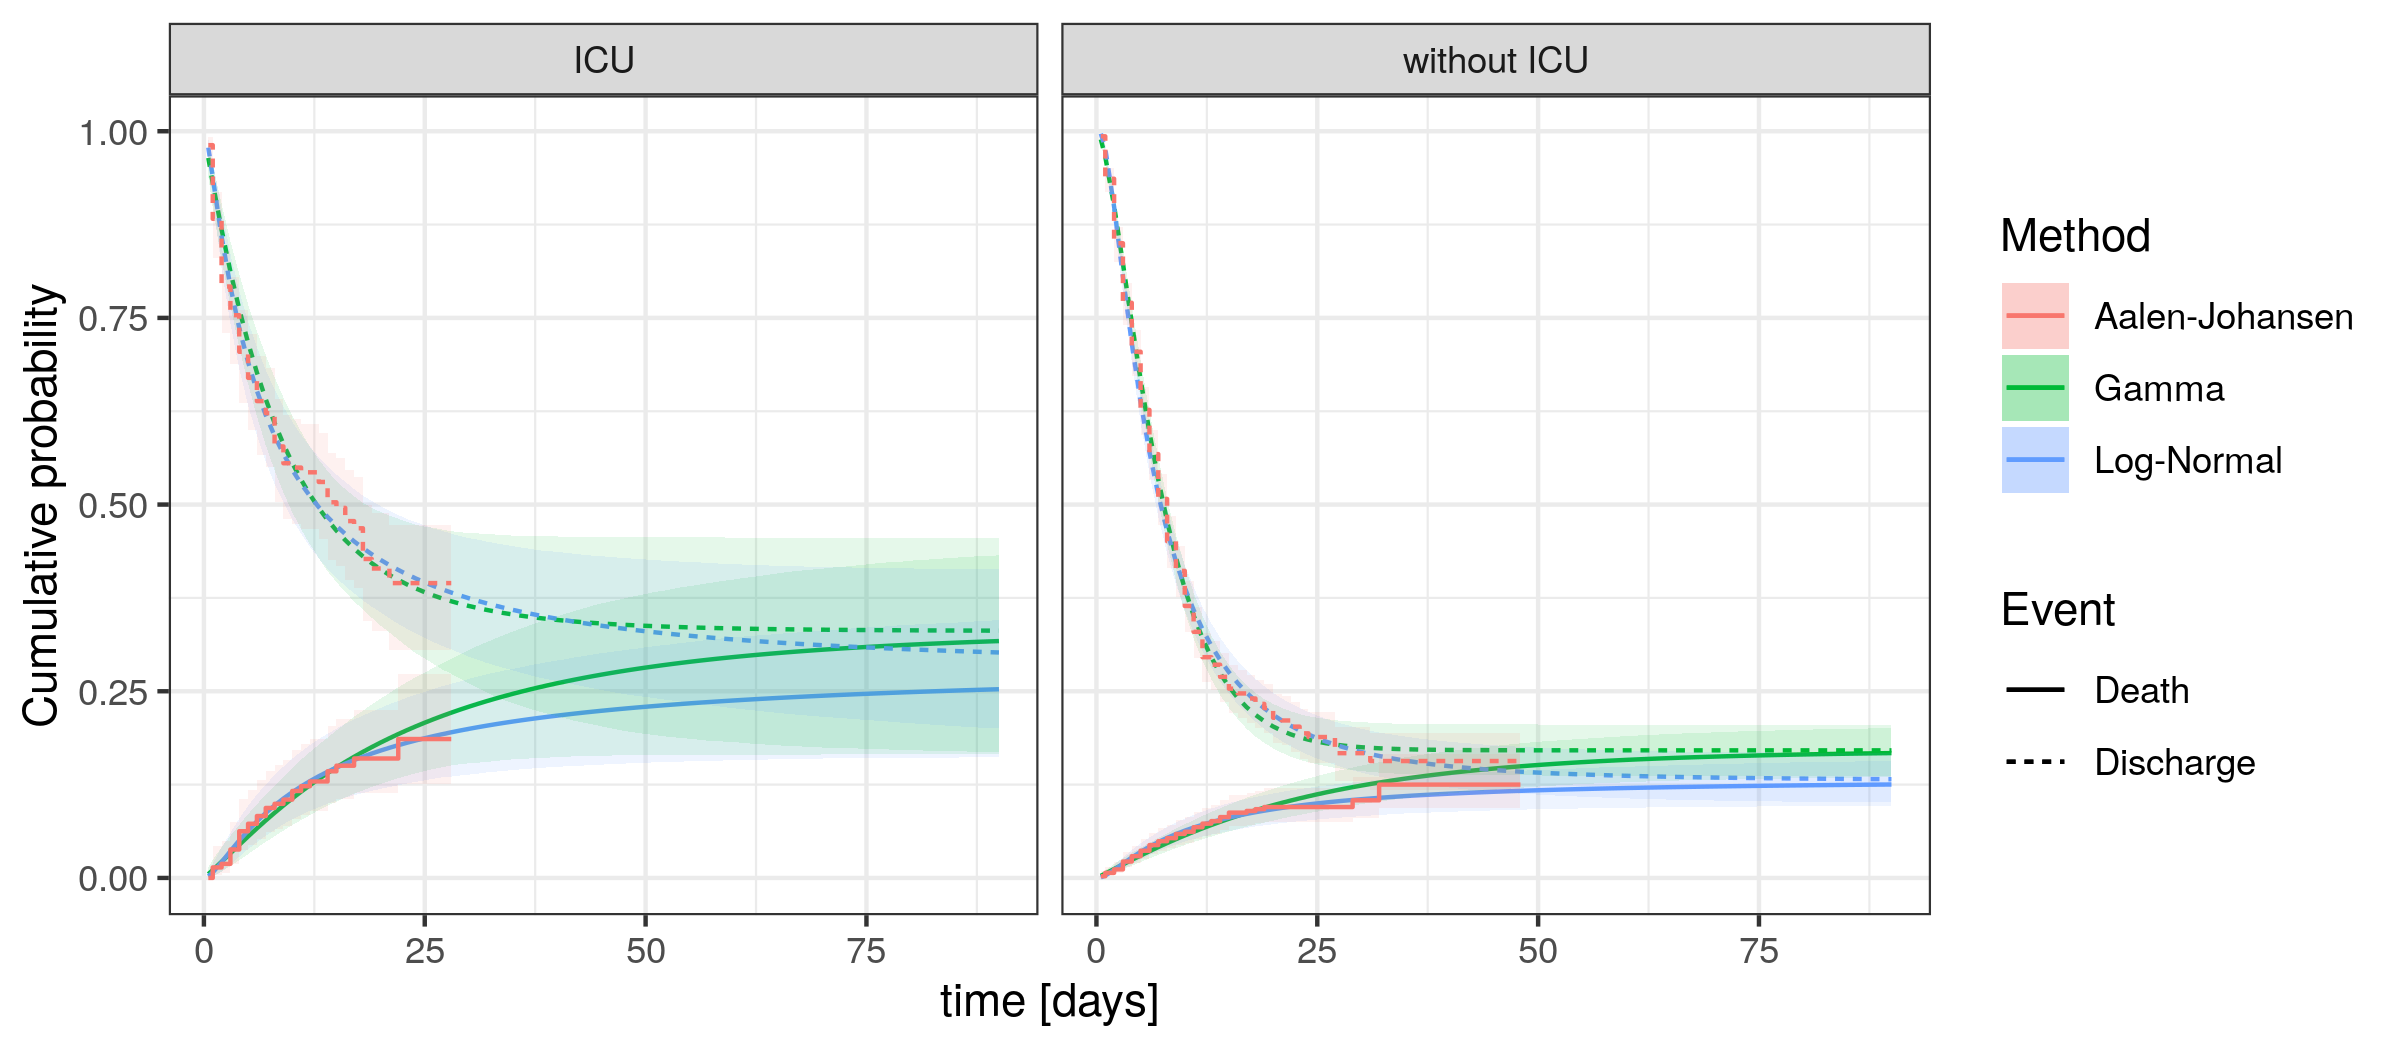
\includegraphics{fig_covid-switzerland-npi/fig_supp/survival_analaysis.png}
    \label{fig:delays}
\end{figure}


Times to death and discharge were best described by log-normal distributions with a single group both for patients having required ICU or not (Fig.~\ref{fig:delays}). When accounting for right-censoring and assuming log-normally distributed times to events, we estimate an overall hCFR of 16.0\% (95\% credible interval, CrI: 12.5-19.8), resulting from a hCFR of 28.1\% (95\% CrI: 16.4-40.9) for patients requiring ICU and 13.0\% (95\% CrI: 9.9-16.6) for patients that did no require it. Estimated hCFRs were slightly higher when assuming gamma-distributed times to events (overall hCFR of 20.3\%, 95\% CrI: 15.9-24.1).


\noindent The distribution of times of hospitalization processes are shown in Fig.~\ref{fig:vdtimes}, and fitted distribution parameters given in Table~\ref{tab:vdparams}.


\begin{table}[t]
\caption[Observed hospitalization time distributions.]{Observed hospitalization time distributions. All times are in days and taken from the date of hospitalization if not specified otherwise. Note that these estimates are biased due to right-censoring of observations and probably under-estimate the true distributions.  Table~\ref{tab:survpars} shows estimates that account for right-censoring.}
\label{tab:vdparams}
\centering
\begin{tabular}{lrrrr}
\toprule
 & mean & sd & mean (logscale) & sd (logscale)\\
\midrule
Time hospitalized & 8.49 & 6.58 & 1.81 & 0.87\\
Time to death & 8.23 & 6.09 & 1.80 & 0.87\\ \addlinespace
Time to discharge without ICU & 6.29 & 4.66 & 1.56 & 0.80\\
Time hospitalized without ICU & 7.35 & 5.79 & 1.68 & 0.85\\
Time to death without ICU & 7.84 & 6.27 & 1.73 & 0.88\\ \addlinespace
Time to ICU & 2.35 & 3.79 & 0.18 & 1.05\\
Time hospitalized with ICU & 13.14 & 7.50 & 2.37 & 0.72\\
Time in ICU & 8.36 & 6.76 & 1.69 & 1.04\\
Time from ICU to discharge & 8.68 & 6.99 & 1.71 & 1.07\\
Time from ICU to death & 6.97 & 4.98 & 1.68 & 0.77\\
\bottomrule
\end{tabular}
\end{table}


\begin{fwtable}
    \centering
    \begin{tabular}{ccccccc}
\toprule
 & & \multicolumn{3}{c}{Log-Normal} & \multicolumn{2}{c}{Gamma}\\ \cmidrule(rl){3-5} \cmidrule(rl){6-7}
Group & Event & median & mean-log & SD-log & scale & shape\\
\midrule
Without ICU & Death & 10 (7.3--16) & 2.3 (2--2.8) & 1.2 (0.95--1.5) & 21 (21--22) & 1.1 (0.83--1.4)\\
 & Discharge & 6.1 (5.6-6.6) & 1.8 (1.7--1.9) & 0.93 (0.87--0.99) & 4.3 (4.4--4.2) & 1.8 (1.6-2)\\ \addlinespace
ICU & Death & 13 (6.2--30) & 2.6 (1.8--3.4) & 1.3 (0.87--1.9) & 21 (12--23) & 1.2 (0.74--1.9)\\
 & Discharge & 6.4 (4.3--9.3) & 1.8 (1.5--2.2) & 1.3 (1.1--1.6) & 9.1 (8.1--11) & 1 (0.75--1.4)\\
\bottomrule
\end{tabular}
\caption[Estimated parameters of hospitalization time distributions.]{Estimated parameters of hospitalization time distributions. These estimates differ from observed values given in Table~\ref{tab:vdparams} by accounting for right-censoring of observations. We report time from hospitalization to discharge or death, and from ICU admission to discharge or death. Estimates were obtained using competing risk survival model as described in section~\ref{sec:crm}. Parameters are given in terms of their posterior mean and 95\% CrI (in parenthesis). For the log-normal distribution the parameters correspond to the mean and SD of the logarithm of the distribution.}
     \label{tab:survpars}
\end{fwtable}

